\documentclass[11pt]{article}
\usepackage{amsmath}  % Math
\usepackage{amssymb}  % Symbols
\usepackage{graphicx} % Images
\usepackage[utf8]{inputenc}
\usepackage[T1]{fontenc}
\usepackage[margin=1in]{geometry}
\usepackage[spanish]{babel}
\usepackage{transparent}
\usepackage{eso-pic}
\usepackage{xcolor}

\graphicspath{{images/}} % Path to images
\newcommand\BackgroundPic{
    \put(0,0){
        \parbox[b][\paperheight]{\paperwidth}{
            \vfill
            \centering
            \transparent{0.2}
\includegraphics[width=\paperwidth]{logo} % your image
            \vfill
        }
    }
}


\title{Informe Negocio Empanadas: \\
  \textit{Empanadas de Juancho, 100\% Legales}}
  \author{Autores: Felipe Colli, Juan Gonzalez, Bastián Ortiz y Javier Robles \thanks{Instituto Nacional General José Miguel Carrera} \\ Curso: \textit{4°H}, Profesor: \textit{Carlos Morales}} % Add your names and course
\date{\today}
\AddToShipoutPicture{\BackgroundPic} % Add background image

\begin{document}

\maketitle
%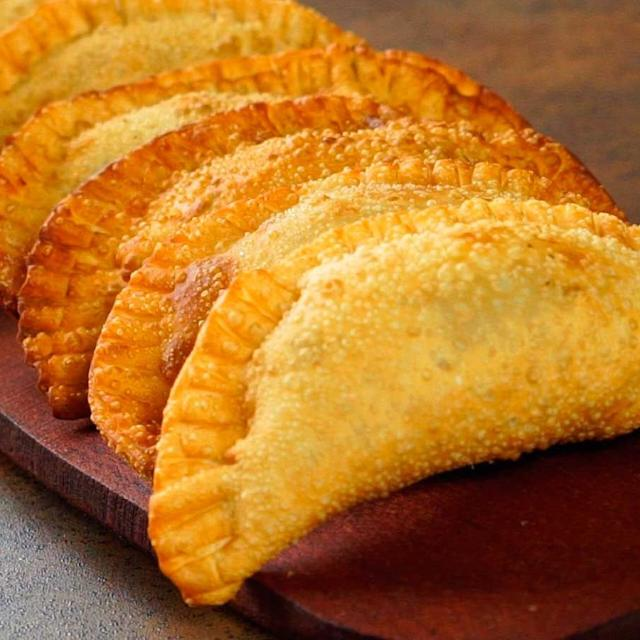
\includegraphics[width=0.95\textwidth]{empanadas} % Logo of the school
\newpage

\tableofcontents
\newpage

\section{Resumen} % Aprox 1/3 de Pagina

\newpage



\section{Introducción} % Max 1 pagina

\newpage



\section{Desarrollo} % 2 - 5 paginas

\newpage



\section{Conclusiones} % Max 1 pagina



\end{document}
